\chapter{Introduction}

Automatic media annotation algorithms essentially assign one or more labels from a search space to a given input image. Figure \ref{fig:with-without-cuenet} shows the various approaches of constructing such a search space for such an algorithm. The traditional approach is shown in \ref{fig:with-without-cuenet}(a). These spaces were limited to a set of labels chosen by an expert, with no way of pruning the search space in case it got very large. The focus was instead on extracting the best features from images, to obtain high overall classification accuracy\cite{turk1991eigenfaces}.

\begin{figure}[t]
\centering
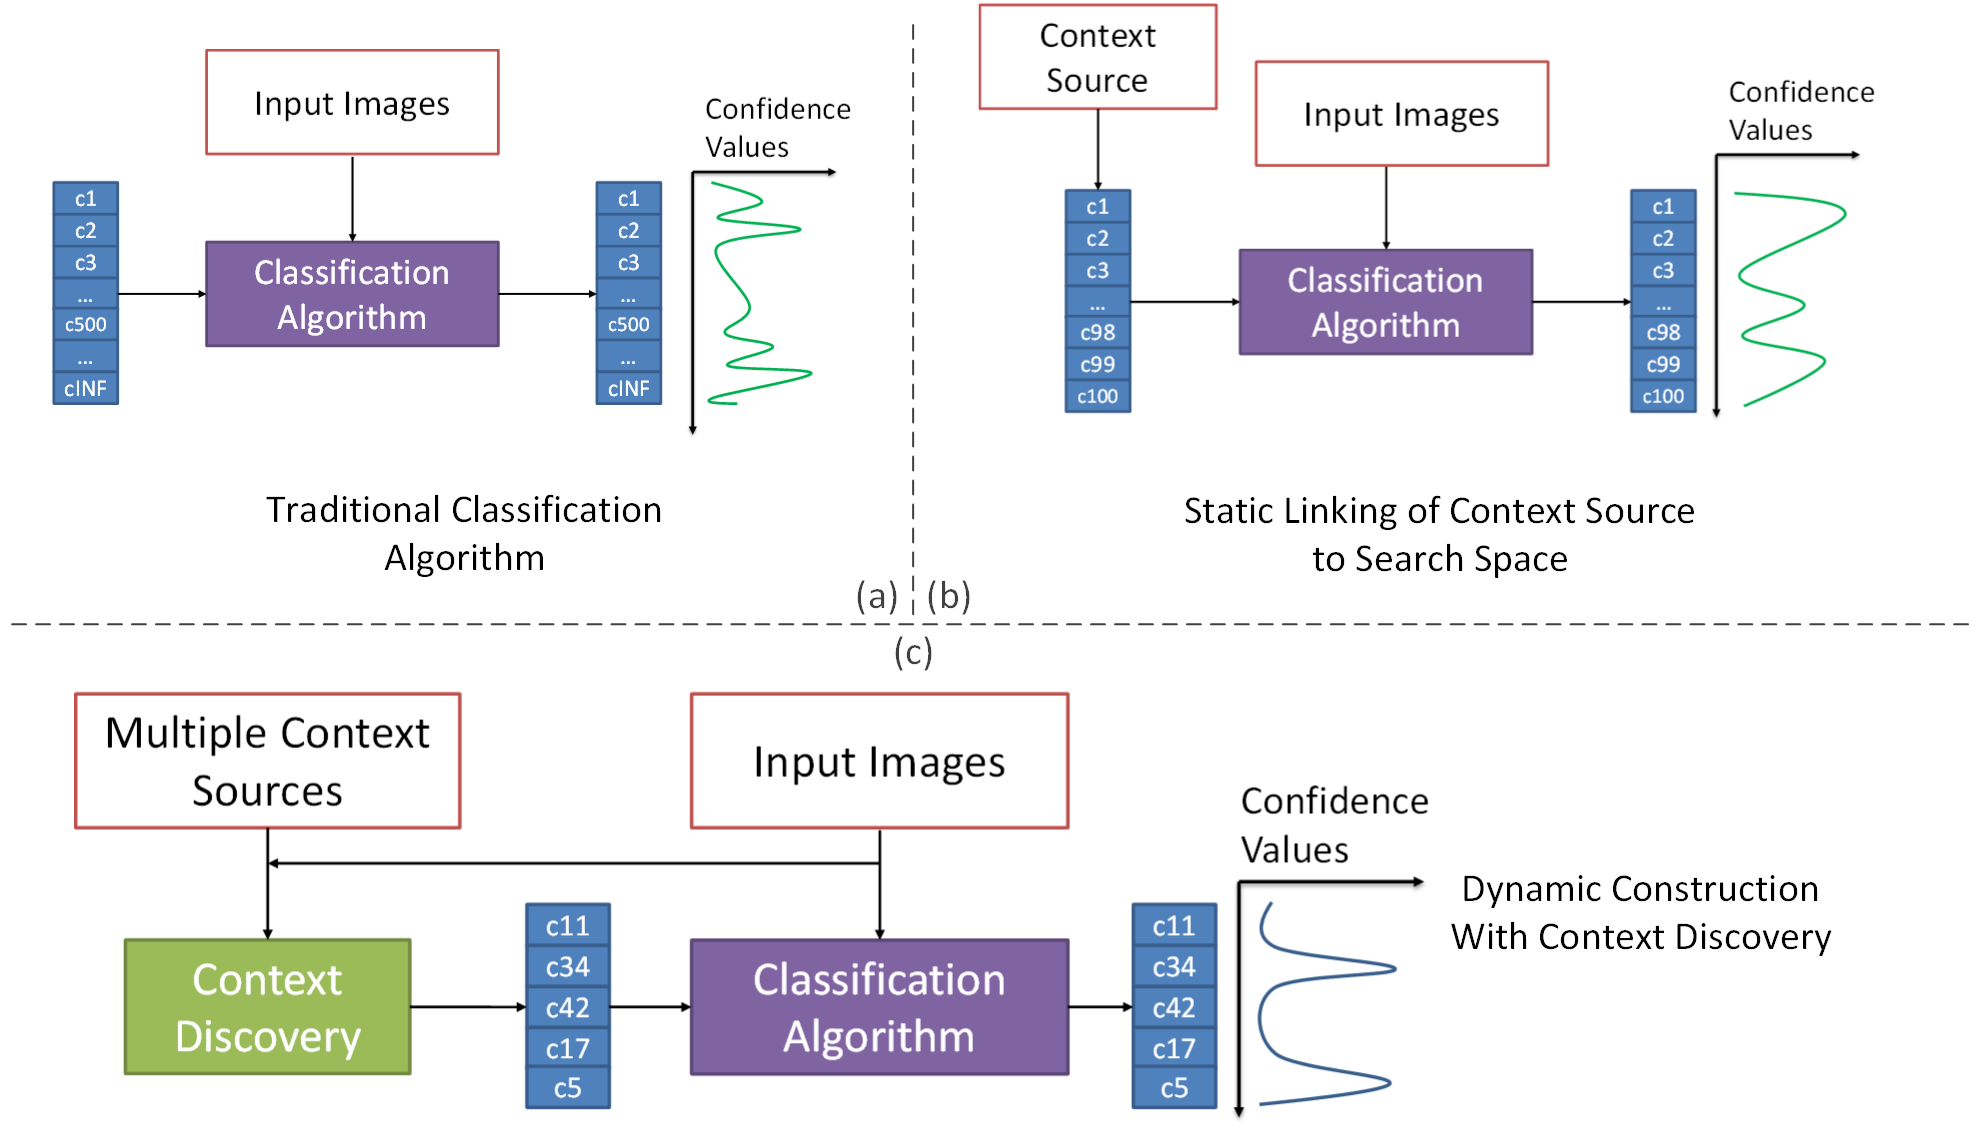
\includegraphics[width=0.95\textwidth]{media/with-without-cuenet-2.png}
\caption{The different approaches in search space construction for a multimedia annotation problem. A traditional classifier setup is shown in (a) where the search space candidates are manually specified. Context is used to generate large static search spaces in (b). The desired framework is shown in (c), which aims to produce small search spaces with many correct annotations.}
\label{fig:with-without-cuenet}
\end{figure}

With the popularity of global social networks and proliferation of mobile phones, information about people, their social connections and day-to-day activities are becoming available at a very large scale. The web provides an open platform for documenting many real world events like conferences, weather events and sports games. With such context sources, the search space construction is being delegated to one or a few sources \cite{henter2012tag, li2012fusing, naaman2005identity, o2009context,  stone2008autotagging} (figure \ref{fig:with-without-cuenet}(b)). These approaches rely on a single \textit{type} of context. For example, time and location information or social network information from Facebook to solve the face recognition problem. We refer to such a direct dependency between the search space and a data source as \textbf{static linking}. Although these systems are meritorious in their own right, they suffer from the following drawbacks: they do not employ multiple sources, and therefore the \textbf{relations} between them. By realizing that these sources are interconnected in their own way, we are able to treat the entire source topology as a network. Our intuition in this work is to navigate this network to progressively discover the search space for a given media annotation problem. Figure \ref{fig:with-without-cuenet}(c) shows how context discovery can provide substantially smaller search spaces for a set of images, which contain a large number of correct tags. A small search space with large number of true positives provides the ideal ground for a classification algorithm to exhibit superior performance.

We present the CueNet framework, which provides access to multiple data sources containing event, social, and geographical information through a unified query interface to extract information from them. CueNet encapsulates our \textbf{Context Discovery Algorithm}, which utilizes the query interface to discover the most relevant search space for a media annotation problem. To ensure a hands-on discussion, we show the use of context discovery in a real world application: face tagging in personal photos. As a case study, we will attempt to tag photos taken at conference events by different users. These photos could contain friends, colleagues, speakers giving very interesting talks, or newly found acquaintances (who are not yet connected to the user through any social network). This makes the conference photos particularly interesting because no single source can provide all the necessary information. It emphasizes the need to utilize multiple sources in a meaningful way.

\begin{figure}[t]
\centering
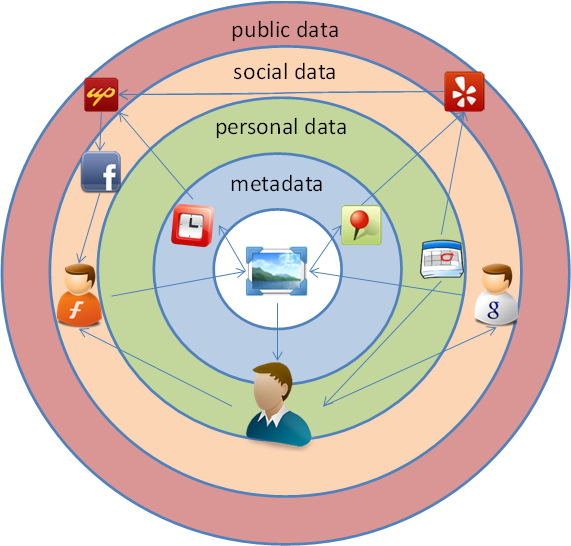
\includegraphics[width=0.65\textwidth]{media/prog-discovery.png}
\caption{Navigation of a discovery algorithm between various data sources.}
\label{fig:prog-discovery}
\end{figure}

Here is an \textbf{example} to illustrate CueNet's discovery process. Let's suppose that Joe takes a photo with a camera that records time and GPS in the photo's EXIF header. Additionally, Joe has two friends. One with whom he interacts on Google+, and the other using Facebook. The framework checks if either of them have any interesting event information pertaining to this time and location. We find that the friend on Google+ left a calendar entry describing an event (a title, time interval and name of the place). The entry also marks Joe as a participant. In order to determine the category of the place, the framework uses Yelp.com with the name and GPS location to find whether it is a restaurant, sports stadium or an apartment complex. If the location of the event was a sports stadium, it navigates to upcoming.com to check what event was occurring here at this time. If a football game or a music concert was taking place at the stadium, we look at Facebook to see if the friend ``Likes" the sports team or music band. By traversing the different data sources in this fashion, the number of people, who could potentially appear in Joe's photograph, was incrementally built up, rather than simply reverting to everyone on his social network or people who could be in the area where the photograph was taken. We refer to such navigation between different data sources to identify relevant contextual information as \textbf{progressive discovery}. The salient feature of CueNet is to be able to progressively discover events, and their associated properties, from the different data sources and relate them to the photo capture event. We argue that given this structure and relations between the various events, CueNet can make assertions about the presence of a person in the photograph. Once candidates have been identified by CueNet, they are passed to the face tagging algorithm (like \cite{facever_pami2010}), which can perform very well as their search space is limited to two candidates.


